\documentclass{article}
\usepackage{tikz}
\usepackage{amsmath,amssymb}
\usetikzlibrary{shapes, arrows, chains}
\tikzstyle{line} = [draw, -latex']
\begin{document}
	
\title{TBW}

\author{G.~A.}

\maketitle

\section{Graph solutions by Evendim}
\subsection{Graph 34}
\begin{figure}[h]\centering{%
	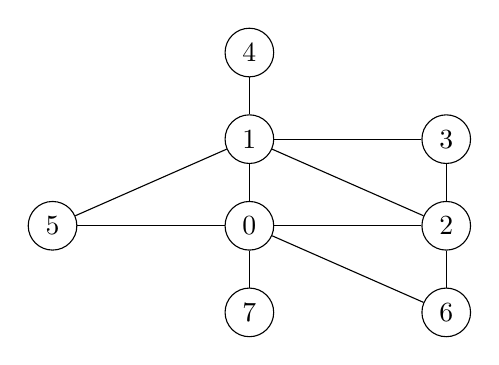
\begin{tikzpicture}
		\def\yn{1.1}
		\def\xn{2.5}
		\node[circle, draw=black] (x0) at (0, 0) {$0$};
		\node[circle, draw=black] (x1) at (0, \yn) {$1$};
		\node[circle, draw=black] (x2) at (\xn, 0) {$2$};
		\node[circle, draw=black] (x3) at (\xn, \yn) {$3$};
		\node[circle, draw=black] (x4) at (0, 2*\yn) {$4$};
		\node[circle, draw=black] (x5) at (-\xn, 0) {$5$};
		\node[circle, draw=black] (x6) at (\xn, -\yn) {$6$};
		\node[circle, draw=black] (x7) at (0, -\yn) {$7$};
		\draw (x0) -- (x1);
		\draw (x0) -- (x2);
		\draw (x0) -- (x5);
		\draw (x0) -- (x6);
		\draw (x0) -- (x7);
		\draw (x1) -- (x2);
		\draw (x1) -- (x3);
		\draw (x1) -- (x4);
		\draw (x1) -- (x5);
		\draw (x2) -- (x3);
		\draw (x2) -- (x6);
	\end{tikzpicture}}
\caption{Graph 34. A solution is given by 3 or 7. The first number (3) is 00000011 in binary, which means
sites 0, 1, have negative signs and form the maximal cut; The other solution ound is 7, 00000111 in binary, which
corresponds to sites 0, 1, and 2 having negative signs and forming the maximal cut. In all cases energy equals -5, fitness 5.}
\end{figure}

\subsection{Graph 35}
\begin{figure}[h]\centering{%
	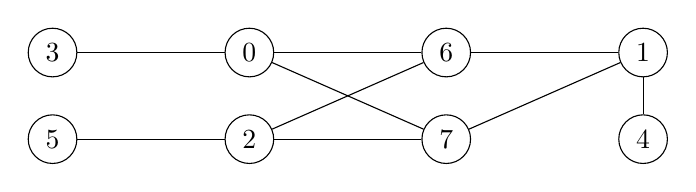
\begin{tikzpicture}
		\def\yn{1.1}
		\def\xn{2.5}
		\node[circle, draw=black] (x0) at (\xn, 0) {$0$};
		\node[circle, draw=black] (x1) at (3*\xn, 0) {$1$};
		\node[circle, draw=black] (x2) at (\xn, -\yn) {$2$};
		\node[circle, draw=black] (x3) at (0, 0) {$3$};
		\node[circle, draw=black] (x4) at (3*\xn, -\yn) {$4$};
		\node[circle, draw=black] (x5) at (0, -\yn) {$5$};
		\node[circle, draw=black] (x6) at (2*\xn, 0) {$6$};
		\node[circle, draw=black] (x7) at (2*\xn, -\yn) {$7$};
		\draw (x0) -- (x3);
		\draw (x0) -- (x6);
		\draw (x0) -- (x7);
		\draw (x1) -- (x4);
		\draw (x1) -- (x6);
		\draw (x1) -- (x7);
		\draw (x2) -- (x5);
		\draw (x2) -- (x6);
		\draw (x2) -- (x7);
	\end{tikzpicture}}
\caption{Graph 35, which is number 4648 in the qaoa paper. A solution is given by 248, which in binary is 00110000, which means
sites 4 and 5 have negative signs and form the maximal cut; energy equals -9, fitness 9.}
\end{figure}

\end{document}

